\documentclass{article}

\usepackage[utf8]{inputenc}
\usepackage[T1]{fontenc}
\usepackage[francais]{babel}
\usepackage{graphicx}
\usepackage{hyperref}
\usepackage{sistyle}

\begin{document}
\title{Algorithmes génétiques et application au problème du voyageur de commerce}
\author{Fabien DUBOIS,\\
   Antoine RATO,\\
   Corentin HEMBISE\\
   \url{https://github.com/dut-info/Algo-Genetique}\\}
\date{\today}

\maketitle

\tableofcontents

\newpage
\section{Principe des algorithmes génétiques}
	\subsection{Introduction}
	Les algorithmes génétiques sont des algorithmes qui se basent sur la sélection naturelle afin de trouver des solutions à un problème d'optimisation, celle - ci est un processus de l'évolution des espèces.
	
	Les individus les plus adaptés à leur environnement, sont plus susceptible de « survivre », alors au fil de nouvelles générations, la population devient meilleur au regard de son environnement.

	En clair, les algorithmes génétiques miment le processus de sélection naturelle pour trouver des solutions efficaces à un problème à un ou plusieurs paramètres.
	Ce sont des algorithmes d'approximation puisqu'il ne permettent pas de trouver la solution optimale à un problème, mais de s'en rapprocher. En outre, ils ont l'avantage de trouver une solution en un temps bien inférieur aux algorithmes déterministes.

    \paragraph{}
	Les termes utilisés dans ce genre de problème sont empruntés de la théorie de l'évolution, ainsi, on parlera :
	\begin{description}
	\item [d'individu :] c'est une solution admissible du problème
	\item [de population :] c'est un ensemble d'individus
	\item [de gène :] c'est une partie d'un individu, une partie du problème
	\item [de génération :] c'est une itération de l'algorithme
	\item [de fonction objectif :] c'est une fonction qui permet de définir qu'un individu est meilleur qu'un autre
	\end{description}

    \paragraph{Pourquoi utiliser des algorithmes génétiques ?}\mbox{}\\
	Dans les problèmes d'optimisation où le nombre de variables est grand, une solution optimale est coûteuse et n'est pas toujours nécessaire, néamoins, le temps de calcul doit être optimisé. Dans cette optique, les algorithmes génétiques sont bien adaptés, puisqu'ils permettent de traiter d'un problème à plusieurs variables efficacement.
	De plus, ce genre d'algorithmes est particulièrement adaptable à différents problèmes.

	\subsection{Principe}
	Les algorithmes de génétique se décomposent en 5 phases :
	\begin{enumerate}
	\item La création d'une population initiale
	\item L'évaluation des individus
	\item La sélection des meilleurs individus
	\item Les croisement et les mutations des enfants
	\item La création d'une nouvelle population
	\end{enumerate}
    \mbox{}\\
    Ensuite, on réitère à partir de la phase $2$ jusqu'à la condition d'arrêt, elle peut être un nombre d'itération ou le moment ou le meilleur individu n'évolue plus.

	\begin{figure}
		\begin{center}
			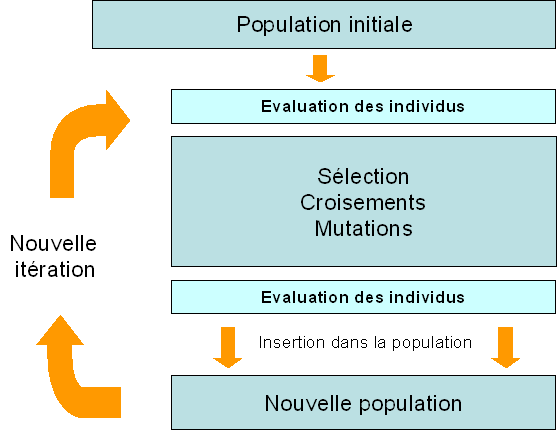
\includegraphics[scale=0.5]{schema_gen.png}
		\end{center}

		\caption{Schéma général d'un algorithme génétique}

		\label{Schéma général d'un algorithme génétique}
	\end{figure}

		\subsubsection{Population initiale}
		La population initiale doit être créer aléatoirement, et chaque individu doit être une solution admissible du problème. Créer aléatoirement la population permet de s'assurer de la diversié de la population. La diversité est un élement important dans ce genre d'algorithmes puisqu'elle permet de ne pas converger vers une solution unique et d'explorer le maximum des solutions du problèmes.

		\subsubsection{Evaluation des individus}
        Chaque individu doit être évaluable, sur une même échelle, on va associer une note à chacun d'entre eux pour pouvoir les comparer. La méthode d'évaluation dépend du problème. L'évaluation est une phase importante lorsque l'on applique un algorithme génétique à un problème multi-critère, puisqu'il faut syntétiser l'ensemble des critères pour ne retourner qu'une "note".

        \subsubsection{Sélection des individus}
        La phase de sélection permet de choisir les individus qui vont survivre à la nouvelle génération et qui seront susceptible de se "reproduire".
        La méthode de sélection doit garder une certaine diversité dans la population, en effet, un individu mauvais \(au regard de sa fonction objectif\), peut donner un enfant très bon après croisement.
        \\
        Plusieurs méthodes existent :

        \paragraph{La sélection élitique}\mbox{}\\
        Ce type de sélection trie les individus d'une géneration par ordre de fitness et choisit les $n/2$ individus les meilleurs. C'est la méthode de sélection la plus simple à implementer. Le problème de cette méthode réside dans le fait qu'elle converge rapidement vers une unique solution, au fil des sélections, la population devient de moins en moins diversifiée.

        \paragraph{La sélection par roulette}\mbox{}\\
        Dans ce type de selection, un individus avec un meilleur fitness qu'un autre à plus de chance d'être choisit. Tous les individus sont placés sur une roulette, plus l'individus à un bon fitness, plus il occupera une grande partie de la roulette. On tire ensuite un emplacement de la roulette au hasard et l'individu correspondant à cet emplacement est sélectionné pour la génération suivante. On réitère le processus jusqu'à obtenir la taille de la nouvelle population souhaitée.

        \paragraph{La sélection par rang}\mbox{}\\
        Ce type de sélection est similaire à la précedente, mais dans ce cas, la probabilité d'être selectionné dépend du rang de l'individus dans la population \(préalablement triée par fitness\). La sélection par roulette présente un inconvénient, si un ou des individus dominent tous les autres, la selection n'assure plus la diversité de la population, la sélection par rang permet de résoudre se problème.

        \paragraph{La sélection par tournoi}\mbox{}\\
        On forme des groupes d'individus aléatoires au seins de la poulation et on selectionne dans chaque groupe, l'individu ayant le meilleur fitness.

        \subsubsection{Croisement des individus}
        La phase de croisement associe deux individus pour créer un ou plusieurs individus enfant, qui partageront les gènes des deux parents. Généralement, on choisit aléatoirement un point de césure $c$ dans la chaine génétique des parents et on copie les $c$ premiers gène du premier parent dans le premier enfant et les gène de $c$ jusque la fin du second parent vers le premier enfant, pour le second enfant, les rôles des deux parents sont inversés.

        \subsubsection{Mutation des individus}
        La mutation consiste à changer aléaoirement un gène d'un individu par un autre gène. Cette phase permet d'éviter la convergence des solutions. Elle s'effectue sur les enfants nouvellements créer et dois avoir une propabilité faible, dans le cas contraire, la recherche deviendrait aléatoire.

\section{Application au porblème du voyageur de commerce}
	\subsection{Définition du problème}
	Le problème est le suivant : 
	\begin{quote}
	Un voyageur de commerce doit visiter $n$ villes données en passant par chaque ville exactement une fois. Il commence par une ville quelconque et termine en retournant à la ville de départ.\\
	Quel chemin faut-il choisir afin de minimiser la distance parcourue ?
	\end{quote}
	
	\subsection{Modélisation du problème}
    Soit :
    \begin{itemize}
        \item $n$ le nombre de villes
        \item $\{v_i\}^{n}$ l'ensemble des villes
        \item $c$ un chemin, c'est à dire une permutation des $n$ villes
        \item $\{D_{d, a}\}^{n, n}$ la distance de la ville $d$ à $a$
    \end{itemize}
    La fonction ocjectif pour un chemin $c$ est : $f(c) = \sum_{i=1}^{n}D_{ c_i c_{(i+1) \bmod n } }$

	Résoudre ce problème en trouvant une solution optimale reviendrais à parcourir l'ensemble des solutions du problème. C'est à dire l'ensemble des chemins, donc toutes les permuations de $c$, soit $n!$ permutations. \\
	Par exemple, pour 10, 30 et 100 villes et si l'on suppose qu'une évaluation d'une permutation coûte 1 \micro s : \\

	\begin{tabular}{ccc}
	\hline
	$n$ & Nombre de permutations & Temps \\
	\hline
	10 & 3 628 800 & 3,6 s\\
	30 & $26 \times 10^{31}$ & $84 \times 10^{15}$ siècles \\
	100 & $93 \times 10^{156}$ & $3 \times 10^{142}$ siècles \\
	\hline
	\end{tabular}
	\\
    Même si pour dix villes une solution optimale reste envisagable, à partir de 30 villes, un algorithme de ce genre serait beaucoup trop long.
	Dans ce cas, l'utilisation d'un algorithme génétique est approprié.

    \subsection{Implementation}

    Dans le cas du problème du voyageur de commerce, un individu représente un chemin, une ville représente un gène qui est modelisé par un entier et une position en x et y.

    \paragraph{Création de la population initiale}: les chemins de départ sont créés aléatoirement, ce qui permet de diversifier au maximum la population initial, et de ne pas se limiter à quelques possibilités.

    \paragraph{Evaluation des chemins}: la fonction objectif calcule pour chaque chemin, la distance totale à parcourir. L'objectif de l'alogorithme est de minimiser cette fonction. Dans notre implémentation, la distance entre deux villes $v_1$ et $v_2$ est donnée par la formule $D_{v_1, v_2} = \sqrt{(v_{1_x}-v_{2_x})^2 + (v_{1_y}-v_{2_y})^2}$

    \paragraph{Selection des chemins}: nous avons implémenté plusieurs méthodes de selection : selection élitique,  selection par roulette, selection par tournoi. \\
    Ce qui nous permettera de comparer les différentes méthodes de selection.

    \paragraph{Croisement des chemins selectionnés}: le croisement de deux chemins parents créés, en fonction du taux de croisement, un ou plusieur individu. Pour un taux de croisement de 1, deux chemins créent 2 enfants, pour 1.5, deux chemins créent en moyenne 1.5 enfants. Ce paramètre nous permettera de faire évoluer la taille de la population au fil des générations.
    Le croisement de deux chemins de taille $m$ s'effectue comme suit :
    \begin{itemize}
    	\item On tire un nombre aléatoire $rand$ entre 1 et $m$
    	\item On copie les villes de 1 à $rand$ du premier parent vers le premier enfant
    	\item On copie les villes du second parent qui ne sont pas dans le premier enfant
    	\item On effectue la même opération pour le second enfant en inversant le rôle des parents
    \end{itemize}

    Cette méthode de croisement nous assure que chaque enfant créé soit un enfant "correct", c'est à dire qu'il soit une permutation des $n$ villes.

    \paragraph{Mutation d'un chemin}: la mutation intervient avec une probabilité de $x \in ]0, 1[$. Le procesus de mutation consite à inverser au hasard deux villes d'un chemin.

	\begin{figure}[!h]
		\begin{center}
			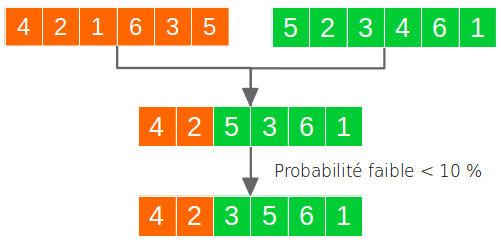
\includegraphics[scale=0.5]{croisement.png}
		\end{center}

		\caption{Schéma d'un croisement et d'une mutation}

		\label{Schéma d'un croisement et d'une mutation}
	\end{figure}

	\subsection{Technique}
	Nous avons implémenté l'algorithme en java, ce qui nous permet d'utiliser le polymorphisme pour par exemple, définir plusieur méthodes de sélection tout en conservant la même logique dans le reste du code. C'est également un langage facilement portable et qui nous est familier.

\section{Résultats}
	\subsection{Paramètrage de l'algorithme}

	Liste des paramètres sur lesquels influer :
	\begin{itemize}
	\item Nombre d'individus initiaux $]1,1000[$
	\item Nombre d'itérations max $]1,5000[$
	\item Nombre de villes $]10,50[$
	\item Méthode de selection (Elistisme, roulette, tournoi)
	\item Taux de mutations $]0,1[$
	\item Taux de selection $]0,1[$
	\end{itemize}

	\subsection{Résultats}

    Afin de comparer nos résultats, nous testé notre programmme sous différentes conditions en faisant varier les paramètres.
    Le graphique ci-contre montre la convergence de l'algorithe au fil des génerations suivant deux méthodes de sélections.
    Les autres paramètres ont été fixés : 500 individus initiaux, 500 itérations max, 30 villes, taux de mutation à 10\% et taux de selection à 50\%
	\begin{figure}[!h]
		\begin{center}
		\makebox[\textwidth][c]{
			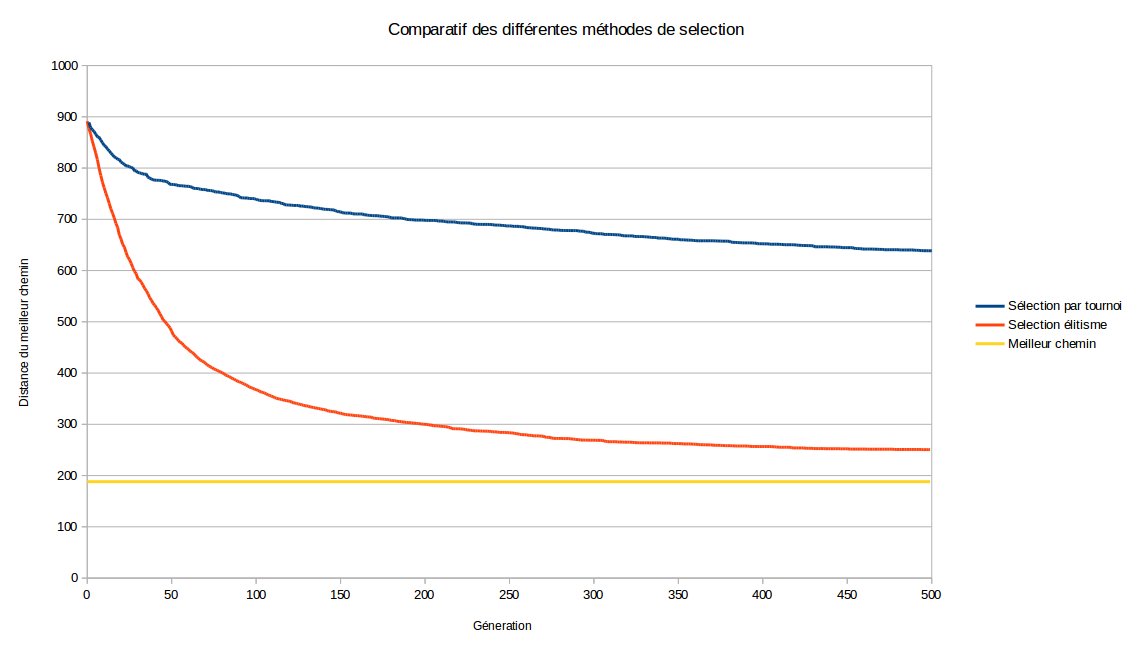
\includegraphics[width=1.4\textwidth]{comparatif.png}
			}
		\end{center}
	\end{figure}

	On remarque que la méthode élitique converge assez rapidement.

	Un second teste nous permet de mesurer l'influence du taux du mutation sur vitesse de l'algorithme. On fait varier le taux de mutation de 0 à 1 avec un pas de 0.01, pour chaque pas, on effectue 60 tests et on fait leur moyenne.
    \begin{figure}[!h]
        \begin{center}
            \makebox[\textwidth][c]{
                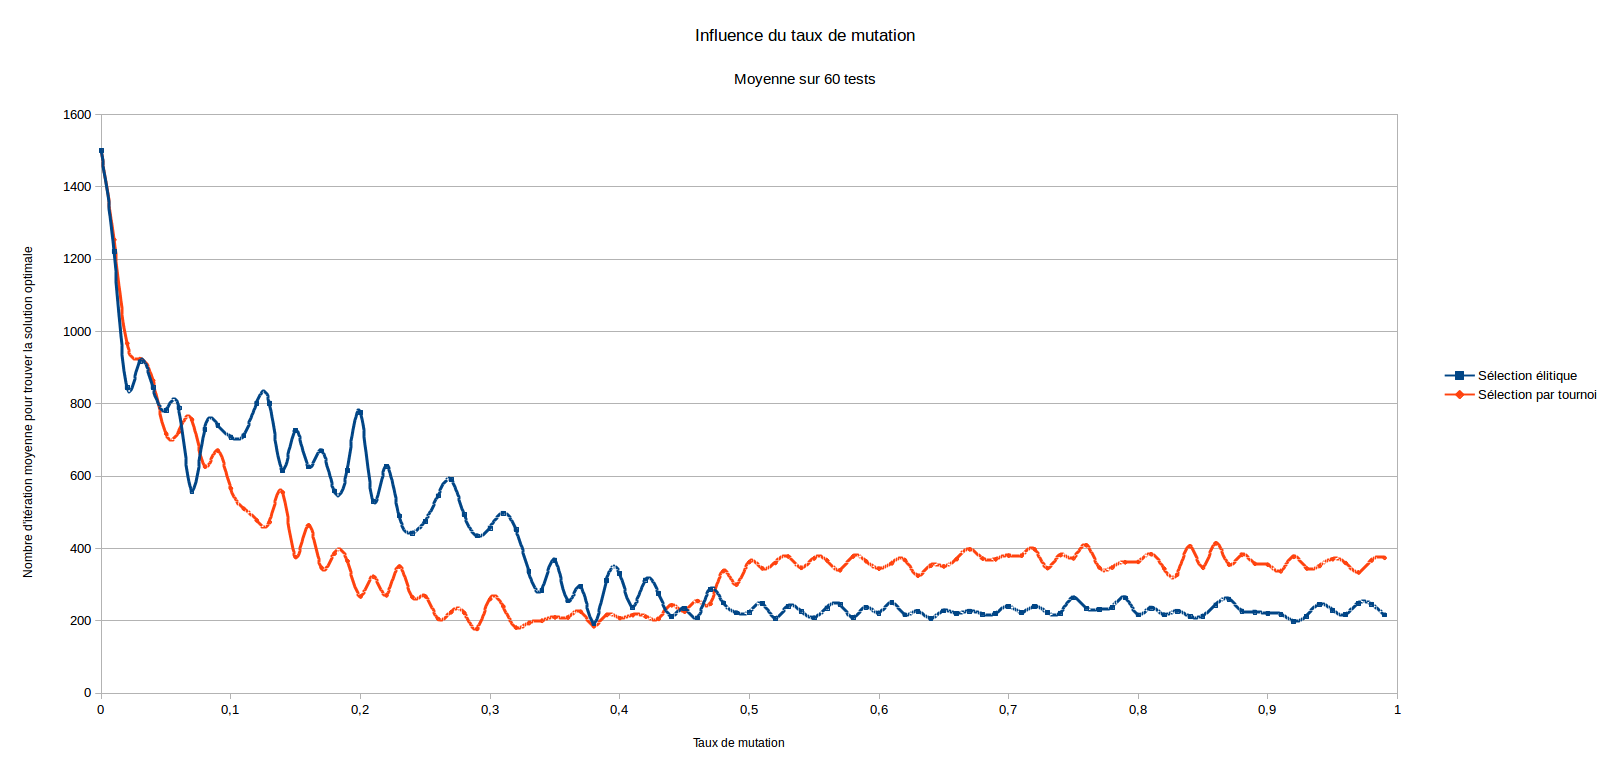
\includegraphics[width=1.4\textwidth]{influence_mutation.png}
            }
        \end{center}
    \end{figure}
    \\
    On remarque que plus le taux de mutation augmente, plus l'on converge vite vers la solution optimale. Néamoins, pour la sélection par tournoi, on remarque une cassure un peu avant 0.5.
    La mutation permet de diversifier la population en ajoutant un facteur aléatoire à la recherche.

\section{Questions}

\begin{enumerate}
\item Quelles sont les 4 étapes d'un algorithme génétique ?
\item Quels sont les avantages des algorithmes génétiques ?
\item En quoi les algorithmes génétiques sont adaptés au problème du voyageur de commerce ?
\end{enumerate}

\section{Références}
	\url{http://khayyam.developpez.com/articles/algo/genetic/}

	\url{http://sis.univ-tln.fr/~tollari/TER/AlgoGen1/node2.html}

	\url{http://www.recherche.enac.fr/opti/papers/thesis/HABIT/main002.html}
\end{document}
